\subsection{What is projectional editing?}

% WIP start

Traditionally programmers write code with text editors, or integrated development environments (IDE), which are basically text editors on steroids.
A projectional editor, also known as structured editor or syntax-directed editor, is a different way to write code.

\subsubsection{parser based editing}

In a traditional, parser-based, development workflow, users use a text editor to represent the program.
Because it is text based then the notation of the language is limited to text.
A grammar is a definition of the formal syntactical rules, or concrete syntax, of a programming language.
The lexer and parser are derived from the grammar.
The text is passed into a text buffer where first a lexer will turn the text into tokens. 
A parser will validates that these tokens, the words of the language, are syntactically correct.
If the tokens are not rejected then the parser will construct first a parse, or concrete syntax, tree and from there, an abstract syntax tree (AST).

An AST is a tree structure that represents the semantic meaning of the source code, stripped of all the syntactic details.
The parser will do some name resolution to take care that references within the source code are represented in the tree. 
This turns the tree into a graph.

Compilers use the AST to do subsequent processing, such as linking, transformation, analysis, type checking, etc.
Modern IDEs, in the background, also parse the code it is displaying to create an AST in order to offer relevant coding assistance.
This assistance is appreciated, because without IDE help learning the concrete syntax of large languages is error prone and exploratory programming is laborious if one has to wait until compilation to discover mistakes.


\subsubsection{projectional definition}

A projectional editor does not parse any text.
In its place, a developer reads and edits the AST through a projected notation.
Her editing gestures immediately and directly manipulate the AST within predefined and fixed layouts.

The principle of projectional editing is familiar to those that use visual programming, like Scratch or Blockly, or graphical modelling tools, such as MetaEdit+.
These tools do not parse pixels to get to their AST. 
They project the underlying models/programs in a view and which they store as the model/AST and not as a plain text equivalent in a traditional programming language.

Projectional editing is the generalization of this idea, with the ability to render multiple representation of the program with a wide range of notation styles.

The projection may be textual. 
It also may be any other notation that can represent the semantic meaning of the code, such as formulas, graphs, or images.
Projections are not just the notation, but also how the user interacts with the projection.
In this sense the definition of the projections and the IDE/UI overlap.

\subsubsection{How projectional editing works}

As shown in figure \ref{fig:projectionalEditing_loop}, a projectional editor has a model or an AST. 
It renders a presentation of the model as a projection. 
The developer performs actions on the projection.
every user editing action is directly mapped on to a change in the AST. 

\begin{figure}[h]
    \centering
    \fbox{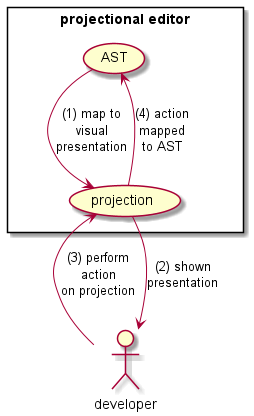
\includegraphics[width=0.95\textwidth]{Sections/images/projections.png}}
    \caption{Projectional editing loop.}
    \label{fig:projectionalEditing_loop}
\end{figure}

To perform the above two things have to be defined by language engineers: The Meta-Model and the editor.

The meta-model, analogous to the abstract syntax, describes the node concepts and connection that can be used to build the, hierarchical structure that is the AST.
This hierarchy can have references to nodes in other branches, so, although named a tree, it is actually a graph.
The AST will be stored independently of the concrete syntax.
The tree is often stored with a database, XML or a proprietary file format.

Rules of the meta-model can further be described through behaviours such as type systems or scoping rules.

Projectional editors avoid the grammars and parsers that serve as the definition of the concrete and abstract syntax in a traditional text based language.
Instead of transforming the concrete to the abstract with parsing, the abstract is transformed to the concrete via a projection engine that uses projection rules.
Editors are a combination of the projection rules and the gestures or actions that will create change request to the AST.
They are analogous to the concrete syntax.

One of the actions can be typing text, however, every string is recognized as it is entered, so there is no tokenizing and the text is being entered into the templates defined in the editor.
The resulting changes are displayed to the developer in a newly derived projection of the underlying AST.

The projection uses graphical elements to represent the representation.
Although often appearing textual, each of the text elements are references to nodes in the AST.

Developers can only interact with the editor via the rigidly controlled code completion menus or gestures and actions. 
    
The AST is directly built from each interaction she has with the editor.
Nodes are creates as instances of the concepts defined in the meta-model.
Each node has it's own unique id and points to it's defining concept.
It is unambiguous.
References are first class and defined by the id rather than resolved by name, as in parser based languages.
Disambiguation happens at time of input, as the developer choses from limited legal inputs.

The separation of the abstract and concrete allows the language engineer to implement multiple projections of the same model, using different notations, each node of the AST taking having the design she envisions.
The pattern used for projection is similar to MVC, so multiple views of the program can be visible and updateable at the same time.

Graphical modelling tools, for example for UML modelling, are specialized implementations of projectional editing.
UML diagrams are not stored as pictures and whose pixels are parsed to create an AST.
Instead the model is stored, often with extra information about visual layout, and the image of the UML is projected to the modeller to edit.
Projectional editing generalizes this approach to projecting any notation defined by the language engineer.


\subsubsection{What advantages does projectional editing bring?}

Projectional editing gives advantages both to the language engineer and the program developers.
There follows, in no particular order, a number of advantages of projectional editing 
 
\paragraph{Exploratory programming}
As with their progenitors, syntax-directed editors, modern projectional editors help guide a developer unfamiliar of a language.
The defined editors with rigid syntax and pre-defined layout mean that only specific cells within the editor can be edited.
This template style means the she does not have to worry about significance of spacing or indentation.
Minutiae of syntactic adornments, such as statement ending semi-colons or enclosing matched brackets, are also not interfering with her exploration of the language space.

When creating code the developer is only presented with legal options within the current context.
As the projection is context aware, relevant actions or options can be suggested and irrelevant ones can be removed.
Thus, it is easier for her to explore which options and actions the language allows her to choose.
Intelligent code completion does not have to be limited to single nodes. 
Whole subtrees can be inserted allowing the developer to explore the larger structures of the language.

\paragraph{Correctness-by-construction}
A projectional editor, by controlling the interaction between the developer and the AST, prevents her from writing syntactically incorrect code.
The whole class of syntactical errors are made impossible, with the developer relieved of having to think about special characters and layout.
Typing and scoping errors are removed by only allowing validly typed and scoped options for the developer.

The developer is only able to select statements that are legal in the context of the location within the AST.
Code does not have to be disambiguated, as this happens at time of entry by the developer.
If there are multiple items that share the same presentation in the editor, the developer chooses the relevant item, resolving the ambiguity to what she means rather than what the parser thinks she means.

\paragraph{Rich notation}
The choice of projection is unconstrained by the restrictions of code that needs to be parsed from a textual source.
This freedom opens up diverse otherwise difficult or impossible to parse notations.
Examples include tabular, mathematical expressions and symbols, diagrams, trees, images, forms, prose, sub- and superscript.
Any visual form or shape that can be mapped to the AST can be used to represent the program in an editor.

With these notations one can better reflect the semantics of the program domain, which should aid comprehension.
Mathematics has a rich history of use of notation.
When writing a DSL for the Mathematics domain, the domain experts can interact with it in the centuries old language of their domain. 

Of course the projections can also be projections of text.  
This is often the appropriate projection type if the developer interacting with the language's domain expertise is parser-based languages.

\paragraph{Mixed notation}
– Notations are more flexible than ASCII/ANSI/Unicode.
Graphical, semi-graphical and textual notations can be mixed and combined.
For example, a graphical tool for editing state machines can embed a textual expression language for editing the guard conditions on transitions.
Since all editors use the same projectional architecture this works seamlessly.
In particular, non-textual notations can be used inside textual notations.
Examples include:
– mathematical symbols embedded in textual programs – tables that contain text or math symbols – tables embedded in textual programs – mathematical symbols embedded in prose – lines, progress bar other other shapes embedded arbitrarily 
ProjEs can also mix different notational styles.
For example, tables can contain textual expressions and mathematical symbols (as in mbeddr’s decision tables), and textual programs can embed graphics.

combination of graphical and textual editing
Graphical, semi-graphical and textual notations can be mixed and combined.
For example, a graphical tool for editing state machines can embed a textual expression language for editing the guard conditions on transitions.

All notations are built on top of the same editor architecture, so they can be freely mixed (math symbols in tables or text in diagrams) while retaining editor support for all of them.

The projection can take on many forms and it is even possible to combine different types of projections, such as including tables inside a textual presentation.
with projectional editing it is natural to combine projections because there is no requirement stating that the syntax should be unambiguous 

\paragraph{Multiple views}
– Since the model is stored independently from its concrete notation, it is possible to represent the same model in different ways simply by providing several projections.
Different viewpoints of the overall program can be stored in one model, but editing can still be viewpoint specific.
Because the model is stored independent of its concrete notation, it is possible to represent the same model in different ways simply by providing several projections.
Different viewpoints [11] of the overall program can be stored in one model, but editing can still be viewpoint specific.
Multiple Editors A single concept can define several editors, and a given program can be edited using any of them.
unconstrained projection, Change notations on fly

Projectional editing, keeping the code in the AST form, and the absence of parsers, brings along several benefits.
• Since the projection is detached from the physical representation of code (AST), authors of languages can define multiple notations and allow the developers to switch between them on the screen.
The language author can define multiple alternative visualizations and let the developer choose one that fits best the task at hand.

multiple notations for same language, choose between readability and writability
multiple simultaneous views
2) change notations on the fly, so you can choose the notation that best suits the problem at hand
Furthermore, the projectional editor is an enabler for multiple notations and for implementing modular and extensible languages.
Several alternative (user-switchable) notations for the same program are also possible.
Notational diversity is crucial for DSLs targeting non-programmers, such as insurance experts, systems engineers or biologists [32]
Because the model is stored independent of its concrete notation, it is possible to represent the same model in different ways simply by providing several projections.
Different viewpoints [7] of the overall program can be stored in one model; editing can be viewpoint or aspect specific.

\paragraph{Language composition}
Its distinguishing feature is its projectional editor, which supports practically unlimited language extension and composition [65]
Since projectional editing disambiguates constructs originating from different languages, it does not require the construction of a unifying parser or the definition of composite grammars.
Languages can be extended with new constructs and new ways to view and edit them.
Since no grammar is used, grammar classes are not relevant, and no syntactic ambiguities can result from the combination of independently developed languages.
If two concepts (possibly defined by different language extensions) with the same syntax are valid in the same location, the user is forced to decide which one to instantiate as she enters the program.
Since a projectional editor never encounters grammar ambiguities, they can support language composition [9].
ProjEs also avoid the problems with compositionality known from grammar-based systems:
ambiguities cannot arise since no grammars are used.
In ProjEs, since no grammars are used, language composition is unlimited (discussed systematically in [8])

Projectional editing has two advantages.
First, it supports flexible composition of languages because the ambiguities associated with parsers cannot happen in projectional editors.
While parser-based systems support language modularization and composition to some degree, it is easy to do and well supported in projectional systems.

Projectional editing, keeping the code in the AST form, and the absence of parsers, brings along several benefits.
• Programming languages can be defined in a modular way, and multiple languages can be easily combined together in a single program or one can extend another.

As a consequence of the projectional editor, very few concrete syntax concerns have to be considered when modularizing and composing languages.

no ambiguities,easy language composition, modular languages, embedded languages , extensible languages
3) combine languages easily
Projectional code does not have to be parsed, so language syntax can have much more options and languages can be freely combined together.
Language composition is easily possible, because languages composition cannot result in ambiguous grammars [1, 19, 20].

projectional editing also supports language composition.  because you never run into ambiguities language composition is much more flexible compared to parser based systems.

Projectional editors have two main advantages, both resulting from the absence of parsing.
Second, they support various ways of language composition [19], typically including modular language extension as well as embedding of unrelated languages into a host language [44, 51]
Language composition refers to using multiple languages in a single program without invasively modifying the definitions of the participating languages.
Extensions can be on arbitrary abstraction levels, thereby integrating modeling and programming and avoiding tool integration issues. 


There is no room for ambiguous or conflicting grammars because there is no need for grammars or parsers at all.
Since projectional editors never encounter grammar ambiguities, they can support language composition [50].
In contrast to parser-based systems, where disambiguation is performed by the parser after a (potentially) complete program has been entered, in projectional editing, disambiguation happens at the time when the user picks a concept from the code completion menu: if two concepts define the same alias, the user resolves the ambiguity.
Furthermore, the projectional editor is an enabler for multiple notations and for implementing modular and extensible languages.
Language composition is easily possible, because composed languages cannot result in ambiguous grammars, a significant issue in classical parser-based systems.
Before projectional editors, technology was the limiting factor requiring unambiguous grammars.

After a user has picked a language construct and it has been instantiated in the AST, a program is never ambiguous: every node points to its defining concept.
This is important, because independently developed languages can be composed in a single program and never lead to structural or syntactic problems, irrespective of the concrete syntax of the participating languages.

For instance, two languages could have overlapping keywords, which parser-based tools could not easily disambiguate (without the need for writing dedicated disambiguation code for the combination of the two languages).
Projectional editing has two major advantages: notational diversity and language composability.


\paragraph{IDE functionality}

The IDE will provide code completion, error checking and syntax highlighting for all languages, even when they are combined.
Because projectional languages by definition need an IDE for editing (it has to do the projection!), language definition and extension always implies IDE definition and extension.
The IDE will provide code completion, error checking and syntax highlighting for all languages, even when they are combined.

faster code completion as there is a smaller set of valid options  , intelligent code completion , low effort to implement mature editor features, syntax highlighting, IDE created by default
Since the context is always known, code-suggestions can be used to explore the possibilities that developers have at the current point in the program.
The number of selectable concepts is reduced by excluding language components.
Also, code-completion is faster when there are less conflicting concept-names.
It is a common behavior in projectional editors to use code-suggestions in order to find out which actions or options are valid in the current context. 
Code-suggestions in projectional editors can reveal possible action and options.

Projectional editor provides intelligent code completion 
An intelligent code completion can be sophisticated and larger parts of code can be inserted automatically, so syntax can be more explanatory without the need of writing more.
The fact that projectional editor manipulates directly with AST allows to implement some editor features that are common in mature IDEs with much less effort.
But the projectional approach goes further: when writing the to-be-generated code, the IDE provides syntax coloring, code completion and error checking for the template code.
This is extremely hard to do for parsed languages, because the parser of the target language has to be embedded into the template language, and IDE services (code completion, syntax coloring, static checks) would have to be merged as well
This aspect is particularly relevant for projectional editors because they usually require users to part from the traditional textual editing experience.


\paragraph{other (language evolution)}
ease of product line development,  no grammar or parser is required,  easy to  migrating when concrete syntax changes, no need to ”extract” the program structure from a flat textual source,
It is also possible to store outof-band data, i.e. annotations on the core model/program.
Examples of this include documentation, pointers to requirements (traceability) [8] or feature dependencies in the context of product lines [9].
It is also possible to store out-of-band data, i.e. annotations on the core model/program, such as documentation, pointers to requirements (traceability), or feature dependencies in the context of product lines.
The following is a list of benefits of projectional editing:
 No grammar or parser is required.
 It is also possible to store out-ofband data, i.e. annotations on the core model/program.
 Examples of this include documentation, pointers to requirements (traceability) [12] or feature dependencies in the context of product lines [13].
 support migrating programs when concrete syntax changes Concrete syntax changes are supported by default with projectional editing without requiring any migration.
 Since only the AST is stored in the model, all concrete syntax elements purely exist in the editor.
 In principle, projectional editing is simpler than parsing, since there is no need to ”extract” the program structure from a flat textual source.
  

            


Projectional editing gives advantages both to the language engineer and the program developers.


Whilst modern IDE's will give you quick feedback on existing supported languages, this is not the case for bespoke DSLs.













%DISADVANTAGES
This idea emerged as early as in 1970s, but it failed to get adopted widely, mostly due to inconvenient and unnatural way of manipulating code.

The freedom in defining the concrete syntax is not problematic for the computer, but it can cause problems for the language user 
Ambiguous syntax is not only a problem for parsers, but a problem that affects humans as well. 
but there are also downsides to this syntax ambiguities do not only affect parsers, but humans as well 

This notational flexibility leads to drawbacks.
In a ParE, a program can always be typed exactly the way it looks by typing the sequence of characters one by one.

ProjE does not support custom layout (SM.6) – the representation is determined completely by the projection rules.

Historically Projectional editors have had useability challenges and weren't used much in practice.  

Traditionally, projectional editors were tedious to use and were hardly adopted in practice.



However, ProjEs have traditionally had two problems.
First, for notations that look textual, users expect that the editing behavior resembles classical text editing as much as possible 
Second, ProjEs cannot store programs in the concrete syntax – otherwise, this syntax would have to be parsed when programs are loaded into the editor.
Instead, programs are stored as a serialized AST, often as XML. 

However, the challenge in projectional editing is making the editing experience convenient and productive.
Traditionally, projectional editors have had a bad reputation because the user experience in editing programs was unacceptable.


Traditionally, projectional editors were hard to use and were not adopted much in practice.

Projectional editing is often considered a drawback because the editors feel somewhat different and the programs are not stored as text, but as a tree (XML).

Traditionally, PEs also have drawbacks, which is why they have not seen much adoption despite their advantages.

The following two drawbacks are the most important.
First, for languages that use a textual syntax, users expect the editor to behave like regular, characteroriented text editors.
Since PEs do not work with sequences of characters, this can be a challenge. 


The second challenge of PEs is infrastructure integration.
PEs do not store programs as text, because this would re-introduce parsing and hence negate the advantages.
Instead, the AST is persisted, typically as XML.
For use in practice, the integration of these XML files with version control systems must be addressed: diff/merge must be supported using the concrete, projected syntax.


Textual source code can be written in any text editor and simply be shared.
However, a projection can still be ambiguous or confusing to the user.
Some projections are really bad and should be rejected, which this paper advocates.

Thus, it is crucial that projectional editors do not negatively impact editing efficiency for textual notations.

This is their weak spot: for textual notations, projectional editors behave differently from what developers know from traditional text editors in terms of the granularity and restrictions of code edits and code selections.

The main drawback of projectional editors is their questionable usability.
Projectional editing can also be used for a syntax that is textual or semi-graphical (mathematical notations for example).
However, since the projection looks like text, users expect interaction patterns and gestures known from "real text" to work (such as cursor movements, inserting/deleting characters, rearranging text, selection).

A projectional editor has to "simulate" these interaction patterns to be usable. 
However, since the projection looks like text, users expect interaction patterns and gestures known from "real text" to work.
For a projectional editor to be useful, it has to "simulate" interaction patterns known from real text.


Because projectional languages by definition need an IDE for editing (it has to do the projection!), language definition and extension always implies IDE definition and extension.


As the examples below will show, projectional editing has a number of intriguing advantages, but there is also a price to pay: this price is the additional effort that goes into defining a nicely usable editor.

This transition requires significant training and it can be a cause of resistance.
By improving the editing experience we can reduce this risk.



Traditionally, projectional editors have also had disadvantages relative to editor usability and infrastructure integration; those are discussed in [3].
One characteristic of projectional editors is that the language structure strictly determines the structure of the code that can be written in the editor.


%EXAMPLES
At the same time, projectional language workbenches like MPS [57] and Intentional [47]

Second, Behringer, Palz, and Berger (2017) present Projectional Editing of Product Lines (PEoPL), a DSL that enables multiple projections for variability mechanisms.

Such editors have existed since the 1980s and gained widespread attention with the Intentional Programming paradigm, which used projectional editing at its core.

Projectional editing, also known as structured editing or syntax-directed editing, is not a new idea; early references go back to the 1980s and include the Incremental Programming Environment [32], GANDALF [35], and the Synthesizer Generator [39].
Work on projectional editors continues today: Intentional Programming [44, 18, 45, 14] is its most well-known incarnation.
Other contemporary tools [20] are the Whole Platform [9], M´as [3], Onion, and MPS [4]

Projectional Editors from the 1980s.
GANDALF [35] and the Incremental Programming Environment (IPE) [32] do not attempt to make editing textual notations efficient; for example, they lack support for linear editing of tree-structured expressions.
The Synthesizer Generator [39] avoids the use of projectional editing at the fine-grained expression level, where textual input and parsing is used.
While this may improve editing efficiency, it risks the advantages of projectional editing, because language composition at the expression level is limited.
Another work that implements and uses a DSL within the Synthesizer Generator [37] concludes: “Program editing will be considerably slower than normal keyboard entry, although actual time spent programming non-trivial programs should be reduced due to reduced error rates.”

The Intentional Domain Workbench (IDW) is the most recent implementation of the Intentional Programming paradigm [44, 18], supporting diverse notations [45, 14].
Since it is a commercial, closed-source project without widespread adoption yet, we cannot easily study it or survey its users.


All contemporary projectional editors are part of language workbenches

An early example of a projectional editor is the Incremental Programming Environment (IPE) [16].
It supports the definition of several notations for a language as well as partial projections, where parts of the AST are not shown.
However, IPE did not address editor usability; to enter 2+3, users first have to enter the + and then fill in the two arguments.
Another early example is GANDALF [17]; the report in [20] states that the authors experienced similar usability problems as IPE: “Program editing will be considerably slower than normal keyboard entry, although actual time spent programming non-trivial programs should be reduced due to reduced error rates.”
The Intentional Programming project [9, 22] has gained widespread visibility and has popularized projectional editing; the Intentional Domain Workbench (IDW) is the contemporary implementation of the approach.
IDW supports diverse notations [7, 23].

Scratch [15] is an environment for learning programming.
It uses a projectional editor, but does not focus on textual editing; it relies mostly on nested blocks/boxes.
So does GP [18].
Textual notations, and thus grammar cells, are not relevant.
Prune [2] is a projectional editor developed at Facebook.
The goal is explicitly to not feel like a text editor; the hypothesis is that tree-oriented editing operations are more efficient than those known from text editors.
While this is an interesting hypothesis, our considerable experience with using projectional editing in real projects has convinced us that this approach is not feasible; hence the work described in this paper.

The Synthesizer Generator [21] is a projectional editor which, at the fine-grained expression level, uses textual input and (regular, textual) parsing.
While this improves usability, it destroys many of the advantages of projectional editing in the first place, because language composition and the use of non-textual notations at the expression level is limited.

Eco [10] relies on language boxes, explicitly delineated boundaries between different languages used in a single program (e.g., the user could define a box with Ctrl-Space).
Each language box may use parsing or projection.
This way, textual notations can be edited naturally, solving the usability issues associated with editing text in a projectional editor.

Lamdu [5], a functional, projectional language (no paper)

. Dataflow visual programming languages, such as Blueprints in the Unreal Engine [2], are often domain-specific.


Early syntax-directed source code editors included Interlisp-D (for Lisp’s limited syntax) and Emily[1] (for PL/I’s rich syntax).

deuce: lightweight structured editing in sketch-n-sketch

Blockly: https://developers.google.com/blockly



An early example of a ProjE is the Incremental Programming Environment (IPE) [4].
Another early example is GANDALF [5], which generates a ProjE from a language specification.

The Synthesizer Generator [7] is also a ProjE.
However, at the fine-grained expression level, textual input and parsing is used.
While this improves usability, it destroys many of the advantages of projectional editing in the first place, because language composition at the expression level is limited.
In fact, extension of expressions is particularly important to tightly integrate an embedded language with its host language [8].

The Intentional Programming [2,3] project has gained widespread visibility and has popularized projectional editing; the Intentional Domain Workbench (IDW) is the contemporary implementation of the approach.
IDW supports diverse notations [9,10].


Language boxes [11] rely on explicitly delineating the boundaries between different languages used in a single program (e.g., the user could change the box with Ctrl-Space).
Each language box may use parsing or projection.













% WIP End